\documentclass[11pt,a4paper]{article}
\usepackage{RaccaStyle-en}
\usepackage{RSMatematica}
\usepackage{RSProgrammazione}

\begin{document}
\thispagestyle{empty}

\rmfamily
\begin{center}
\ \\
\vspace{2cm}

\LARGE{\textcolor[rgb]{1,0,0}{REPORT FOR THE PROJECT\\ for the exam of\\BIG DATA SCIENCE AND MACHINE LEARNING}\\}
\hrulefill \\
\huge{\textcolor[rgb]{1,0,0}{\ \\Calculus of Napier's number}\\}
\hrulefill \\
\vspace{1.5cm}

\Large{Academic Year 2021/2022
\\ \ \\
Professors: GABRIELE GAETANO FRONZÉ\\
FEDERICA LEGGER\hspace{4.2cm} \\
\hspace{-1cm}SARA VALLERO\hspace{15.2cm} \\
\ \\ \ \\ 
Candidate: RACCA ELEONORA}

\vspace{5cm}
\begin{figure}[h]
\centering
	\includegraphics[width=0.3\textwidth]{../Images/ScuolaDottoratoUnito.pdf} 
	\hspace{5mm} 
	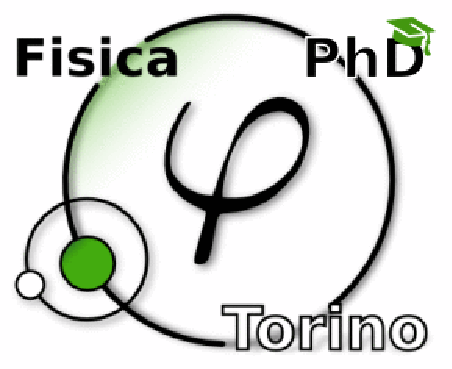
\includegraphics[width=0.3\textwidth]{../Images/ScuolaDottoratoFisica.pdf}
\end{figure}

\end{center}

\newpage
\section{Introduction}
Sequential programming can be very time consuming.

\subsection{Napier's number}

\section{Parallel execution in for loops}

\section{Avoiding race conditions}

\section{Conclusions}


\end{document}
